Pada bagian ini dibahas perancangan sistem \emph{motion} yang berfungsi untuk
mengatur dan mengoordinasikan pergerakan robot secara keseluruhan. Sistem ini
dirancang agar mampu menghasilkan pola gerak yang stabil, presisi, dan adaptif
terhadap hasil komputasi kinematika yang dijalankan pada Jetson Nano.
Implementasi \emph{motion} dilakukan menggunakan kerangka \emph{Robot Operating
System} (ROS), yang menyediakan arsitektur modular berbasis \emph{node} sehingga
setiap proses kontrol gerak, sinkronisasi antar kaki, dan pembangkitan
trajektori dapat dijalankan secara paralel dan saling terintegrasi. Bahasa
pemrograman yang digunakan adalah C++, dipilih karena memiliki kinerja tinggi,
dukungan luas terhadap pustaka ROS, serta efisiensi dalam pengolahan data
numerik untuk komputasi kinematika dan kontrol gerak.

\subsection{Perancangan Gerak Kaki Robot}
\begin{figure} [H] \centering
  % Nama dari file gambar yang diinputkan
  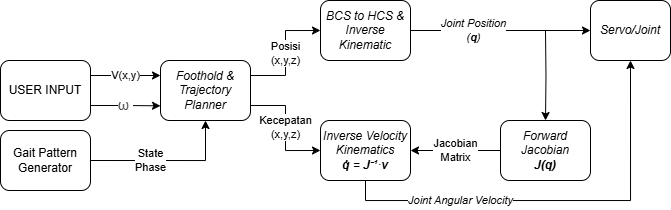
\includegraphics[scale=0.6]{gambar/Perancangan_gerak_kaki.drawio.png}
  % Keterangan gambar yang diinputkan
  \caption{Diagram Alir Perancangan Gerak Kaki Robot}
  % Label referensi dari gambar yang diinputkan
  \label{fig:diagram_alir_perancangan_gerak_kaki}
\end{figure}

Blok \textit{User Input} berfungsi sebagai sumber utama perintah gerak bagi
sistem kontrol kaki robot. Pada bagian ini, pengguna memberikan masukan berupa
kecepatan linear $(v_x, v_y)$ dan kecepatan rotasi $(\omega)$ yang menentukan
arah serta laju pergerakan tubuh robot. Nilai kecepatan translasi mengatur gerak
maju, mundur, maupun ke samping, sedangkan kecepatan rotasi mengatur seberapa
cepat robot berputar terhadap sumbu vertikalnya. Informasi dari \textit{user
input} ini menjadi referensi bagi \textit{Foothold \& Trajectory Planner} untuk
menghitung posisi dan lintasan gerak kaki agar sesuai dengan keinginan pengguna.
Dengan demikian, blok ini berperan sebagai antarmuka utama antara operator dan
sistem gerak robot, memastikan perintah yang diberikan dapat diterjemahkan
menjadi gerakan yang stabil dan terkoordinasi.

Selain blok \emph{user input}, terdapat pula blok \emph{gait pattern generator}
berfungsi sebagai pengatur ritme pergerakan tiap kaki robot selama berjalan.
Modul ini menentukan kapan suatu kaki harus berada pada fase stance (menapak)
dan kapan harus fase swing (mengayun). Dengan demikian, gait generator menjadi
dasar koordinasi gerak seluruh kaki agar pola langkah tetap stabil dan sinkron.

Implementasi yang digunakan memuat dua jenis gait, yaitu stand dan tripod,
yang didefinisikan sebagai berikut:
\begin{itemize}
  \item \textbf{Stand Gait:} digunakan saat robot diam. Semua kaki memiliki
  duty factor = 1, artinya seluruh kaki selalu dalam fase stance.
  \item \textbf{Tripod Gait:} digunakan saat robot bergerak. Enam kaki dibagi
  menjadi dua kelompok tripod yang bergerak bergantian, dengan phase offset
  bernilai [0, 0.5, 0, 0.5, 0, 0.5]. Artinya, kaki 1, 3, dan 5 berada pada fase
  yang sama, sedangkan kaki 2, 4, dan 6 memiliki pergeseran fase \(180^\circ
  \)terhadap kelompok pertama.
\end{itemize} 
Secara matematis, tiap kaki $i$ memiliki \textit{fase waktu gait} $\phi_i(t)$ yang dinyatakan sebagai:
\begin{equation}
\phi_i(t) = \left( \frac{t - \text{phase\_offset}_i \cdot T}{T} \right) \bmod 1
\end{equation}
dengan:
\begin{itemize}
    \item $T$ adalah \textit{total period} dari gait (misalnya 0.8 s untuk tripod),
    \item $\text{phase\_offset}_i$ adalah pergeseran fase kaki ke-$i$,
    \item dan $t$ adalah waktu berjalan dari sistem.
\end{itemize}

Nilai fase $\phi_i(t) \in [0, 1)$ merepresentasikan posisi relatif siklus langkah dari kaki ke-$i$. 
Kemudian, untuk menentukan status langkah digunakan faktor tugas (\textit{duty factor}) $\beta_i$, yaitu proporsi waktu \textit{stance} dalam satu siklus:
\begin{equation}
\text{kaki } i =
\begin{cases}
\text{stance}, & \phi_i(t) < \beta_i \\
\text{swing}, & \phi_i(t) \geq \beta_i
\end{cases}
\end{equation}

Dengan formulasi ini, setiap kaki memiliki waktu \textit{stance} dan
\textit{swing} yang konsisten terhadap periodenya, serta sinkron antar kaki
sesuai dengan nilai \textit{phase offset}-nya. Proses pembaruan fase dilakukan
secara periodik mengikuti waktu sistem, sehingga nilai fase setiap kaki selalu
mencerminkan posisi terkini dalam siklus langkah. Informasi fase ini kemudian
dimanfaatkan pada \emph{foothold \& trajectory planner} untuk menghitung posisi
target kaki selama gerakan berlangsung.

Setelah fase gerak dari setiap kaki diperbarui oleh \textit{gait generator},
proses berikutnya adalah penentuan posisi pijakan kaki atau \textit{foothold
planning}. Pada tahap ini, sistem memperkirakan posisi pijakan berikutnya
(\textit{next foothold}) berdasarkan kecepatan tubuh yang diperintahkan (\(v_x,
v_y, \omega_z\)) serta durasi langkah yang sedang berlangsung. Setiap kali
terjadi transisi dari fase \textit{stance} ke \textit{swing}, posisi pijakan
baru dihitung dengan mempertimbangkan pergeseran tubuh akibat translasi dan
rotasi selama satu periode \textit{stance}. Secara matematis, perpindahan
translasi tubuh dapat ditulis sebagai:
\begin{equation}
\Delta_{\text{trans}} = 
\begin{bmatrix}
v_x t_{\text{stance}} \\
v_y t_{\text{stance}} \\
0
\end{bmatrix},
\end{equation}
sedangkan perpindahan akibat rotasi tubuh diberikan oleh:
\begin{equation}
\Delta_{\text{rot}} = 
t_{\text{stance}} (\boldsymbol{\omega} \times \mathbf{r}_{\text{tip}}),
\quad \text{dengan} \quad 
\boldsymbol{\omega} = 
\begin{bmatrix}
0 \\ 0 \\ \omega_z
\end{bmatrix}.
\end{equation}
Kedua komponen perpindahan tersebut digunakan untuk menentukan posisi pijakan
baru melalui pergeseran setengah dari total perpindahan tubuh, yaitu:
\begin{equation}
\mathbf{p}_{\text{next}} = 
\mathbf{p}_{\text{tip}} + 
\frac{1}{2} (\Delta_{\text{trans}} + \Delta_{\text{rot}}),
\quad
\mathbf{p}_{\text{current}} = 
\mathbf{p}_{\text{tip}} - 
\frac{1}{2} (\Delta_{\text{trans}} + \Delta_{\text{rot}}).
\end{equation}

Dengan formulasi ini, pijakan berikutnya akan berada pada posisi yang seimbang
terhadap pergerakan tubuh, sehingga lintasan kaki dapat direncanakan secara
halus dan stabil. Posisi \textit{foothold} hasil perhitungan ini kemudian
digunakan oleh \textit{trajectory planner} untuk menghasilkan lintasan ayun
(\textit{swing trajectory}) dari posisi pijakan saat ini menuju pijakan
berikutnya selama fase \textit{swing} berlangsung.

Setelah posisi \textit{foothold} ditentukan, langkah selanjutnya adalah
menghasilkan lintasan (\textit{trajectory}) gerak kaki dari titik awal menuju
titik akhir secara halus. Proses ini dilakukan oleh \textit{Trajectory Planner},
yang menerima masukan berupa posisi awal $\mathbf{p}_{\text{start}}$, posisi
akhir $\mathbf{p}_{\text{end}}$, dan tinggi langkah $h$. Untuk menginterpolasi
lintasan tersebut digunakan sebuah variabel fase (\textit{phase variable}) yang
didefinisikan sebagai
\begin{equation}
r = \frac{1 - \cos(\pi t_r)}{2},
\label{eq:r_def}
\end{equation}
dengan $t_r = \dfrac{t}{T_\text{swing}}$ merupakan rasio waktu terhadap durasi
langkah (\textit{stance time}). Nilai $r$ meningkat dari $0$ hingga $1$ secara
halus dengan profil sinusoidal, sehingga menghasilkan gerakan yang mulus pada
awal dan akhir langkah. Turunan pertama terhadap waktu diberikan
oleh
\begin{align}
\dot{r} &= \frac{\pi}{2} \sin(\pi t_r) \, \dot{t_r}
\end{align}
Variabel $r$ berfungsi sebagai parameter interpolasi antara titik awal dan
titik akhir lintasan kaki. Posisi ujung kaki (tip) pada setiap waktu dihitung
dengan persamaan
\begin{equation}
\mathbf{p}(r) = (1 - r)\mathbf{p}_{\text{start}} + r\,\mathbf{p}_{\text{end}},
\end{equation}
dengan penambahan komponen vertikal yang mengikuti kurva sinusoidal untuk
membentuk lintasan ayunan (swing) kaki:
\begin{equation}
p_z(r) = p_{z,\text{start}} + h \sin(\pi r).
\end{equation}
Dengan demikian, lintasan lengkap posisi tip kaki dinyatakan sebagai
\begin{equation}
\mathbf{p}(r) = 
\begin{bmatrix}
(1 - r)p_{x,\text{start}} + r p_{x,\text{end}} \\
(1 - r)p_{y,\text{start}} + r p_{y,\text{end}} \\
(1 - r)p_{z,\text{start}} + r p_{z,\text{end}} + h \sin(\pi r)
\end{bmatrix}.
\end{equation}


Kecepatan lintasan diperoleh dari turunan pertama terhadap waktu, yaitu
\begin{equation}
\mathbf{v}(r) =
\begin{bmatrix}
\bigl(p_{x,\text{end}} - p_{x,\text{start}}\bigr)\,\dot{r} \\
\bigl(p_{y,\text{end}} - p_{y,\text{start}}\bigr)\,\dot{r} \\
\bigl(p_{z,\text{end}} - p_{z,\text{start}}\bigr)\,\dot{r} + h\pi\cos(\pi r)\,\dot{r}
\end{bmatrix}.
\label{eq:velocity_component}
\end{equation}

Dalam implementasi ini, nilai percepatan tidak digunakan secara eksplisit,
sehingga hanya posisi dan kecepatan yang dikembalikan oleh fungsi perencana
lintasan. Perumusan ini menghasilkan lintasan kaki yang halus dan simetris,
dengan kecepatan nol di awal (r=0) dan akhir langkah (r=1), yang sesuai
dengan gerakan alami saat berjalan.

Setelah diperoleh posisi dan kecepatan kaki dalam sistem koordinat global hasil
perencanaan trajektori, langkah selanjutnya adalah melakukan konversi koordinat
dari \textit{Body Coordinate System} (BCS) menuju \textit{Hip Coordinate System}
(HCS). Konversi ini diperlukan karena perhitungan \textit{inverse kinematics}
dilakukan berdasarkan sistem koordinat lokal pada masing-masing kaki robot.

Dalam sistem BCS, titik pusat tubuh robot didefinisikan sebagai titik asal
koordinat, dengan sumbu \(y_B\) mengarah ke depan robot, sumbu \(x_B\) ke arah
lateral kanan, dan sumbu \(z_B\) ke arah vertikal atas. Setiap kaki ke-\(i\)
memiliki sistem koordinat HCS dengan titik asal pada sendi pangkal (\textit{hip
joint}) dan orientasi sumbu \(z_H\) sejajar dengan sumbu \(z_B\). Posisi pangkal
kaki ke-\(i\) terhadap pusat tubuh ditentukan oleh jarak radial \(d_h\)
(\textit{hip diagonal offset}) dan sudut orientasi \(\theta_i\) terhadap sumbu
\(x_B\).

Transformasi dari sistem HCS ke BCS dinyatakan dengan transformasi homogen sebagai berikut:
\begin{equation}
\mathbf{T}_{\text{HCS}\rightarrow\text{BCS}, i} =
\begin{bmatrix}
\mathbf{R}_{z}(\theta_i) & \mathbf{t}_i \\
\mathbf{0}_{1\times3} & 1
\end{bmatrix},
\label{eq:T_HCS_BCS}
\end{equation}
dengan
\begin{equation}
\mathbf{R}_{z}(\theta_i) =
\begin{bmatrix}
\cos\theta_i & -\sin\theta_i & 0 \\
\sin\theta_i & \cos\theta_i & 0 \\
0 & 0 & 1
\end{bmatrix},
\quad
\mathbf{t}_i =
\begin{bmatrix}
d_h \cos\theta_i \\[4pt]
d_h \sin\theta_i \\[4pt]
0
\end{bmatrix}.
\end{equation}
Matriks rotasi \(\mathbf{R}_{z}(\theta_i)\) menyatakan orientasi sistem HCS
terhadap BCS akibat perbedaan arah penempatan kaki pada tubuh robot. Vektor
translasi \(\mathbf{t}_i\) menunjukkan posisi pangkal sendi kaki ke-\(i\)
terhadap titik pusat tubuh robot.

Untuk mengubah titik atau vektor dari sistem tubuh (BCS) ke sistem kaki (HCS),
digunakan transformasi invers dari persamaan \eqref{eq:T_HCS_BCS}:
\begin{equation}
\mathbf{T}_{\text{BCS}\rightarrow\text{HCS}, i} 
= 
\mathbf{T}_{\text{HCS}\rightarrow\text{BCS}, i}^{-1}
=
\begin{bmatrix}
\mathbf{R}_{z}^{T}(\theta_i) & -\mathbf{R}_{z}^{T}(\theta_i)\mathbf{t}_i \\
\mathbf{0}_{1\times3} & 1
\end{bmatrix}.
\label{eq:T_BCS_HCS}
\end{equation}

Dengan demikian, posisi ujung kaki hasil perencanaan trajektori
\(\mathbf{p}_{\text{BCS}}\) dapat dikonversi menjadi posisi dalam sistem lokal
kaki (\(\mathbf{p}_{\text{HCS}}\)) menggunakan relasi:
\begin{equation}
\mathbf{p}_{\text{HCS}, i} 
= 
\mathbf{R}_{z}^{T}(\theta_i)\left(\mathbf{p}_{\text{BCS}} - \mathbf{t}_i\right).
\label{eq:position_conversion}
\end{equation}

Sedangkan kecepatan ujung kaki dalam sistem HCS diperoleh melalui transformasi
rotasi yang sama tanpa translasi, karena translasi tidak memengaruhi kecepatan
linear:
\begin{equation} \mathbf{v}_{\text{HCS}, i} =
\mathbf{R}_{z}^{T}(\theta_i)\mathbf{v}_{\text{BCS}}. \label{eq:
velocity_conversion} \end{equation}

Secara fisis, proses ini memastikan bahwa posisi dan kecepatan ujung kaki yang
semula dinyatakan relatif terhadap tubuh robot kini direpresentasikan dalam
kerangka masing-masing kaki. Hal ini menjadi langkah awal yang krusial sebelum
dilakukan proses \textit{inverse kinematics}, di mana sudut tiap sendi akan
dihitung berdasarkan posisi ujung kaki \(\mathbf{p}_{\text{HCS}, i}\) dalam
sistem lokalnya masing-masing.

\subsection{Perancangan Gerak Lengan Robot}

